\documentclass[aspectratio=169,xcolor={dvipsnames,table}]{beamer}

% Packages
\usepackage{tikz}
\usepackage{amsmath,amssymb,amsfonts}
\usepackage{bbm}
\usepackage{booktabs}
\usepackage{graphicx}
\usepackage{tcolorbox}
\tcbuselibrary{skins}

% Colors (Modern & Colorful)
\definecolor{CyanPrimary}{RGB}{0,166,214}
\definecolor{DarkBlue}{RGB}{10,37,64}
\definecolor{AccentPink}{RGB}{236,72,153}
\definecolor{AccentGreen}{RGB}{16,185,129}
\definecolor{LightBg}{RGB}{248,250,252}

% Beamer Theme
\mode<presentation>{
    \usetheme{Boadilla}
    \usecolortheme{orchid}
}
\setbeamercolor{structure}{fg=CyanPrimary}
\setbeamercolor{frametitle}{bg=LightBg, fg=DarkBlue}
\setbeamercolor{title}{bg=CyanPrimary, fg=white}
\setbeamercolor{block title}{bg=CyanPrimary!15!white, fg=DarkBlue}
\setbeamercolor{block body}{bg=LightBg, fg=black}
\setbeamercolor{item}{fg=CyanPrimary}
\setbeamercolor{alerted text}{fg=AccentPink}

% Font
\usefonttheme{professionalfonts}

% Custom title slide layout
\setbeamertemplate{title page}{
    \vspace*{1cm}
    \begin{center}
        {\usebeamercolor[fg]{title}\usebeamerfont{title}\Huge\bfseries\inserttitle\par}
        \vspace{0.5cm}
        {\usebeamerfont{subtitle}\large\textcolor{DarkBlue}{\insertsubtitle}\par}
        \vspace{0.8cm}
        {\usebeamerfont{author}\insertauthor\par}
        \vspace{0.2cm}
        {\usebeamerfont{institute}\small\insertinstitute\par}
        \vspace{0.5cm}
        {\usebeamerfont{date}\small\insertdate\par}
    \end{center}
}

% Remove navigation symbols
\setbeamertemplate{navigation symbols}{}

\title{Learning with Little Side Information}
\subtitle{Classification from Partitioned Datasets with Test-Time Side Information}
\author{Manish Kumar Singh \and Suhas S. Kowshik \and Ankur A. Kulkarni}
\institute{IIT Bombay \and Microsoft \and IIT Bombay}
\date{2026}

% Math operators from paper
\newcommand{\R}{\mathbb{R}}
\newcommand{\E}{\mathbb{E}}
\newcommand{\lamz}{\lambda_z}
\newcommand{\ws}{w^\star}
\newcommand{\vs}{v^\star}
\newcommand{\us}{u^\star}
\newcommand{\whl}{\hat{w}_\lambda}
\newcommand{\wslz}{w^\star_{\lambda,z}}
\newcommand{\wsz}{w^\star_z}
\newcommand{\ph}{\hat{\phi}}

\begin{document}

\begin{frame}
    \titlepage
\end{frame}

\begin{frame}{Outline}
    \tableofcontents
\end{frame}

\section{Motivation}
\begin{frame}{Motivation -- University Admissions}
    \begin{columns}[T]
        \begin{column}{0.48\textwidth}
            \begin{tcolorbox}[colback=CyanPrimary!5,colframe=CyanPrimary,title=\textbf{The Scenario}]
                \begin{itemize}
                    \item A \textbf{primary university} predicts applicants' aptitude from profiles.
                    \item At test time, an applicant also discloses a \textbf{secondary university's decision} (\alert{side information}).
                    \item Goal: Leverage this decision to improve the primary university's accuracy.
                \end{itemize}
            \end{tcolorbox}
        \end{column}
        \begin{column}{0.48\textwidth}
            \begin{tcolorbox}[colback=AccentPink!5,colframe=AccentPink,title=\textbf{The Challenge}]
                \begin{itemize}
                    \item No candidate in historical data has \textbf{both} admission outcomes simultaneously.
                    \item Training data is \textbf{partitioned}: features + primary labels \emph{or} features + secondary labels.
                    \item The joint distribution $(X,Y,Z)$ is \alert{unlearnable} from partitioned data.
                \end{itemize}
            \end{tcolorbox}
        \end{column}
    \end{columns}
\end{frame}

\section{Problem Setup}
\begin{frame}{Problem Setup: Partitioned Dataset}
    \textbf{Spaces}: Feature $\mathcal{X} \subset \R^d$, Label $\mathcal{Y} = \{-1,1\}$, Side Info $\mathcal{Z} = \{-1,1\}$.
    
    \vspace{0.5cm}
    \begin{tcolorbox}[colback=LightBg, colframe=DarkBlue, title=\textbf{Partitioned Training Data}]
        \begin{itemize}
            \item Primary dataset $D = \{(x_i, y_i)\}_{i=1}^n$ (missing $z_i$)
            \item Secondary dataset $S = \{(x_j, z_j)\}_{j=n+1}^{n+m}$ (missing $y_j$)
        \end{itemize}
        \small All samples drawn i.i.d. from the joint $(X,Y,Z)$, but \textbf{labels and side info are never observed together}.
    \end{tcolorbox}
    
    \vspace{0.3cm}
    \textbf{Goal}: At test time, given $(x, z)$, predict label $\hat{y}$ using a classifier learned from \emph{both} datasets.
\end{frame}

\begin{frame}{Key Definitions: Generative Models}
    We employ three logistic regression classifiers thresholded at $0.5$:
    
    \vspace{0.3cm}
    \begin{enumerate}
        \item \textbf{Side-Info Classifier}: Predicts $Z$ from $X$.
        \[ \phi_u(x) = 2\mathbbm{1}_{\{\sigma(u_c + u_x^\top x) > 0.5\}} - 1 \quad \rightarrow \quad \textbf{Optimal:} \ \us \]
        
        \item \textbf{Primary Classifier}: Predicts $Y$ from $X$ alone.
        \[ \psi_v(x) = 2\mathbbm{1}_{\{\sigma(v_c + v_x^\top x) > 0.5\}} - 1 \quad \rightarrow \quad \textbf{Optimal:} \ \vs \]
        
        \item \textbf{Composite Classifier}: Predicts $Y$ from $(X, Z)$.
        \[ \pi_w(x,z) = 2\mathbbm{1}_{\{\sigma(w_c + w_x^\top x + w_z z) > 0.5\}} - 1 \quad \rightarrow \quad \textbf{Optimal:} \ \ws \]
    \end{enumerate}
\end{frame}

\section{Algorithm}
\begin{frame}{Algorithm: Learning with Side Information}
    \textbf{Two-Stage Imputation Procedure:}
    \vspace{0.3cm}
    
    \begin{tcolorbox}[colback=white, colframe=CyanPrimary, coltitle=DarkBlue, title=\textbf{Stage 1: Imputation Model}]
        Learn $X \to Z$ mapping $\hat{u}$ by minimizing regularized empirical risk on dataset $S$. This defines the side-info classifier $\ph$.
    \end{tcolorbox}
    
    \begin{tcolorbox}[colback=white, colframe=AccentGreen, coltitle=white, title=\textbf{Stage 2: Composite Classifier}]
        \begin{enumerate}
            \item For each $(x_i, y_i) \in D$, \textbf{impute} $z_i = \ph(x_i)$.
            \item Train regularized composite classifier $\whl$ on $D$ using imputed $z_i$.
            \item Regularization: $\lambda_c |w_c|^2 + \lambda_x \|w_x\|^2 + \textcolor{AccentPink}{\lamz} |w_z|^2$.
        \end{enumerate}
    \end{tcolorbox}
    
    \centering
    \alert{$\lamz$ is the critical hyperparameter controlling trust in imputed $Z$.}
\end{frame}

\section{Main Results}
\begin{frame}{Main Result: Upper Bound on Excess Risk}
    \begin{block}{Theorem (Main Theorem)}
    With high probability, the excess population risk is bounded by:
    \begin{align*}
        R(\whl) - R(\ws) \;\leq\;& \underbrace{\mathcal{O}\left(\frac{1}{\sqrt{n}}\right)}_{\text{Estimation Error}} \\
        &+\; \underbrace{\min\left\{\mathcal{O}(\lamz), \mathcal{O}(1)\right\} \cdot \big(T(\vs) - R(\ws)\big)}_{\text{Regularization Bias}} \\
        &+\; \underbrace{\min\left\{\mathcal{O}\left(\frac{1}{\lamz}\right), \mathcal{O}(1)\right\} \cdot \left(\mathcal{O}\left(\frac{1}{\sqrt{m}}\right) + L(\us)\right)}_{\text{Imputation Error}}
    \end{align*}
    \end{block}
\end{frame}

\begin{frame}{The $\lamz$ Trade-Off}
    \begin{columns}[T]
        \begin{column}{0.48\textwidth}
            \begin{tcolorbox}[colback=AccentGreen!5,colframe=AccentGreen,title=\textbf{Small $\lamz$ (Full Trust)}]
                \begin{itemize}
                    \item Encourages use of side info $Z$.
                    \item \textbf{Regularization Bias $\downarrow$}
                    \item \textbf{Imputation Error $\uparrow$}
                    \item Best when $Z$ is informative and predictable from $X$.
                \end{itemize}
            \end{tcolorbox}
        \end{column}
        \begin{column}{0.48\textwidth}
            \begin{tcolorbox}[colback=AccentPink!5,colframe=AccentPink,title=\textbf{Large $\lamz$ (No Trust)}]
                \begin{itemize}
                    \item Ignores side info $Z$ in prediction.
                    \item \textbf{Regularization Bias $\uparrow$}
                    \item \textbf{Imputation Error $\downarrow$}
                    \item Best when $Z$ is noisy or poorly imputed.
                \end{itemize}
            \end{tcolorbox}
        \end{column}
    \end{columns}
\end{frame}

\section{Bang-Bang Behavior}
\begin{frame}{Bang-Bang Optimality of Regularizer}
    \begin{tcolorbox}[colback=CyanPrimary!5,colframe=CyanPrimary,title=\textbf{Key Takeaway}]
        For large $n, m$ and $L(\us) \leq 1$, the optimal regularizer $\Lambda_z^\star$ is either \textbf{$\infty$} or \textbf{$0$}.
    \end{tcolorbox}
    
    \begin{itemize}
        \item \textbf{Regime I}: If side info is noisy/uninformative $\implies \Lambda_z^\star = \infty$ (completely ignore).
        \item \textbf{Regime II}: If side info is clean/informative $\implies \Lambda_z^\star = 0$ (fully trust).
        \item \alert{There is no middle ground!} The model should never partially trust the imputed side information in the asymptotic limit.
    \end{itemize}
\end{frame}

\section{Fundamental Limits}
\begin{frame}{Lower Bound: A Fundamental Limitation}
    \begin{block}{Theorem (Lower Bound on Excess Risk)}
        For \textbf{any} learning algorithm $A$ trained on partitioned dataset $(D, S)$, there exists a valid joint distribution of $(X,Y,Z)$ such that:
        \[ \mathbb{P}\left[ R(A(D,S)) - R(\ws) > 0.19 \right] \geq \frac{1}{2} \]
    \end{block}
    
    \vspace{0.3cm}
    \textbf{Proof Idea}:
    \begin{itemize}
        \item Construct two joint distributions with \textbf{identical marginals} $(X,Y)$ and $(X,Z)$.
        \item Partitioned datasets only reveal marginals!
        \item No algorithm can distinguish the two distributions, yielding an irreducible error term regardless of infinite $n, m$.
    \end{itemize}
\end{frame}

\section{Simulations}
\begin{frame}{Simulation Results}
    \begin{columns}
        \begin{column}{0.45\textwidth}
            \textbf{Setup:}
            \begin{itemize}
                \item 100 random Gaussian mixture distributions for $(X,Y,Z)$
                \item $m=1000$, $n=4000$
                \item Candidate $\lamz \in \{10^{-2}, 10^{-1}, \dots, 10^5\}$
            \end{itemize}
            \vspace{0.5cm}
            \textbf{Observation:}
            Optimal $\lamz$ aggressively concentrates at the extreme edges! This verifies the theoretical \alert{bang-bang behavior}.
        \end{column}
        \begin{column}{0.5\textwidth}
            \centering
            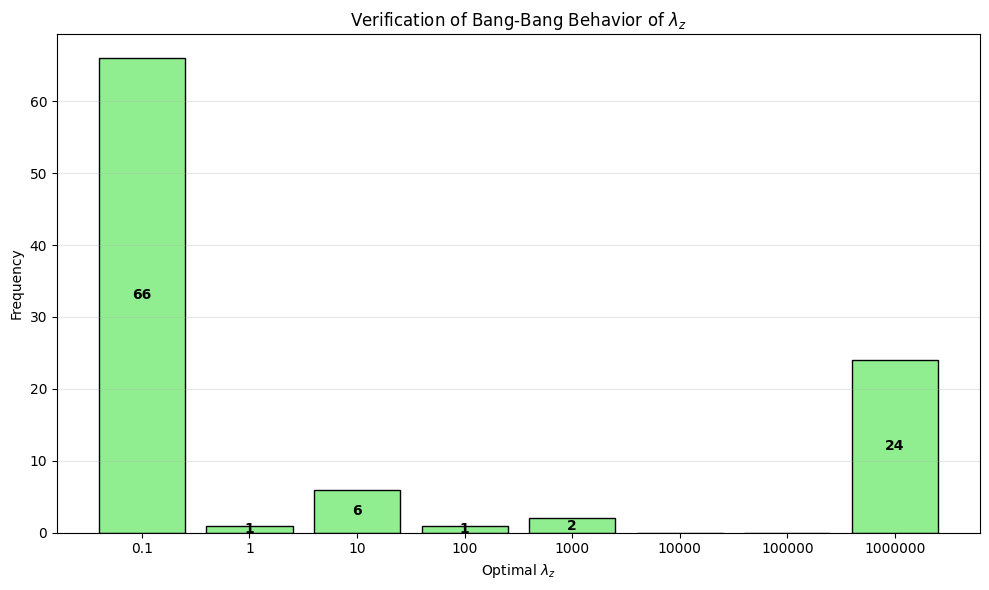
\includegraphics[width=\textwidth]{lambda_frequency.png}
        \end{column}
    \end{columns}
\end{frame}

\begin{frame}{Conclusion}
    \begin{itemize}
        \item \textbf{The Core Issue}: Classification using side information from partitioned datasets where features, labels, and side info are never jointly observed.
        \item \textbf{The Method}: A two-stage imputation algorithm utilizing a critical regularization hyperparameter $\lamz$.
        \item \textbf{The Math}: Explicit upper bounds on excess risk featuring a tension between estimation and imputation.
        \item \textbf{The Surprise}: The optimal choice of $\lamz$ is \emph{binary} --- full trust or complete ignorance.
        \item \textbf{The Limit}: Even infinite datasets cannot close the gap due to unlearnable joint distributions.
    \end{itemize}
    
    \vspace{0.5cm}
    \centering
    \Large \textbf{Thank You!}
\end{frame}

\end{document}
